\section{Fundamental Notations}\label{subsec:auxdefs}
In this section, we present the fundamental notations used in our formalization.
Some of them are auxiliary functions, others are however important ones as they
directly implement our algorithm for method resolution.

\subsection{Auxiliary functions}
To begin with, we introduce the following basic functions. 

\begin{flalign*}
	& \rhd \textit{Definition of } I[m\ \kwoverride\ J]: & \\
	& \bullet I[m\ \kwoverride\ J] = \method{I_e}{m}{I_x}{x}{J}{e_0} & \\
	& \indent\indent \textrm{with: }
	  \kwinterface \; I \; \kwextends \; \overline{I} \; \{ \method{I_e}{m}{I_x}{x}{J}{e_0} \ldots \} & \\
	& \bullet I[m\ \kwoverride\ J] = \absmethod{I_e}{m}{I_x}{x}{J} & \\
	& \indent\indent \textrm{with: }
	\kwinterface \; I \; \kwextends \; \overline{I} \; \{ \absmethod{I_e}{m}{I_x}{x}{J} \ldots \} & \\
\end{flalign*}
Here $I[m\ \kwoverride\ J]$ is basically a directly lookup for method $m$ in the body of $I$, where such a method
overrides $J$. The method can be either concrete or abstract, and the body of definition is returned. Notice that
by our syntax, $I[m\ \kwoverride\ I]$ is looking for the originally-defined method $m$ in $I$.

\begin{flalign*}
	& \rhd \textit{Definition of } \prune(set): & \\
	& \bullet \prune(set) = \{I \in set \; | \; \nexists J \in set\setminus I, J <: I\} &
\end{flalign*}
The $\prune$ function takes a set of
types, and filters out those that have subtypes in the same set. In the returned set,
none of them has subtyping relation to one another, since all super types have been removed.

\begin{flalign*}
	& \rhd \textit{Definition of } \canOverride(m, I, J): & \\
	& \bullet \canOverride(m, I, J) = True & \\
	& \indent\indent \textrm{with: } I[m\ \kwoverride\ I] = I_e \; m(\overline{I_x} \; \overline{x}) \; \kwoverride \; I \ldots & \\
	& \hspace{.77in} J[m\ \kwoverride\ J] = I_e \; m(\overline{I_x} \; \overline{y}) \; \kwoverride \; J \ldots &
\end{flalign*}
$\canOverride$ just checks that two original $m$ in $I$ and $J$ have the same type.

\begin{figure*}[t]
    \begin{mathpar}
    \inferrule* [left=]
        {  \mostSpecific(m, I_d, I_s) = \{I\} \\
            \mostSpecificOverride(m, I_d, I) = \{J\} \\
            \kwinterface \; J \; \kwextends \; \overline{J} \; \{\method{I_e}{m}{I_x}{x}{I}{e_0}\ldots\}}
        {\mbody(m, I_d, I_s) = (J, \overline{I_x} \; \overline{x}, I_e \; e_0)}
    
    \inferrule* [left=]
        {  \mostSpecific(m, I_d, I_s) = \{I\} \\
            \mostSpecificOverride(m, I_d, I) = \{J\} \\
            \kwinterface \; J \; \kwextends \; \overline{J} \; \{\absmethod{I_e}{m}{I_x}{x}{I}\}}
        {\mbody(m, I_d, I_s) = (J, \overline{I_x} \; \overline{x}, I_e \; \o)}

    
   
    \end{mathpar}
    \caption{Auxiliary functions.}\label{fig:auxfunc}
\end{figure*}

\begin{figure*}[t]
    \centering
    \vspace{-1ex}
    \begin{tabular}{ccc}
        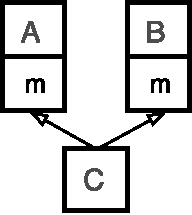
\includegraphics[width=1.5cm]{pics/P1.pdf}\hspace{4pt} &
        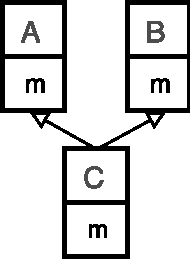
\includegraphics[width=1.5cm]{pics/P2.pdf}\hspace{4pt} &
        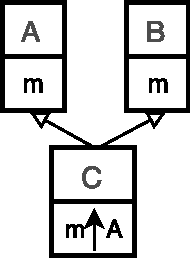
\includegraphics[width=1.5cm]{pics/P3.pdf}\hspace{4pt} \\
        (a) $\mbody(m,C,A) = (A,...)$\ \ \  & (b) $\mbody(m,C,A) = (C,...)$\ \ \  & (c) $\mbody(m,C,A) = (C,...)$
    \end{tabular} \\
   \begin{tabular}{cc}
    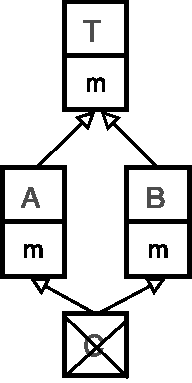
\includegraphics[height=3cm]{pics/P4.pdf}\hspace{4pt} &
    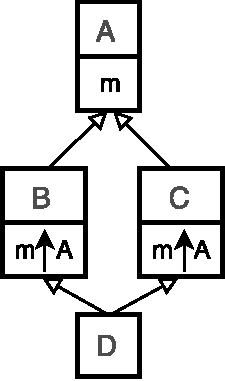
\includegraphics[height=3cm]{pics/P5.pdf}\hspace{4pt} \\ 
    (d) $\mbody(m,D,A) = \keyword{undefined}$\ \ \  & (e) $\mbody(m,D,A) = \keyword{undefined}$
   \end{tabular}
    \caption{Examples on $\mbody$. ``$\uparrow$'' stands for hierarchical overriding.}\label{fig:examplesmbody}
    %\saveSpaceFig
\end{figure*}

\subsection{$\mostSpecific$ and $\mostSpecificOverride$}

$\mostSpecific$ and $\mostSpecificOverride$ are two core functions for the method lookup algorithm. Generally,
$\mostSpecific(m, I, J)$ finds the set of most specific interfaces where $m$ is originally defined, they should be above $I$ and
along path $J$. ``Along path $J$'' means one should be either a subtype or a super type of $J$. Finally with $\prune$
the overridden interfaces will be filtered out.

\begin{flalign*}
	& \rhd \textit{Definition of } \mostSpecific(m, I, J): & \\
	& \bullet \mostSpecific(m, I, J) = \prune(origins) & \\
	& \indent\indent \textrm{with: } origins = \{K \mid \subt{I}{K}, \textrm{ and } \subt{K}{J} \; \lor \; \subt{J}{K}, &\\
	& \hspace{1.62in} \textrm{ and } K[m\ \kwoverride\ K] \textrm{ is defined} \} &
\end{flalign*}
By the definition, an interface belongs to $\mostSpecific(m, I, J)$ if and only if:
\begin{itemize}
	\item It originally defines $m$;
	\item It is a super type of $I$;
	\item It is either a super type or a subtype of $J$ (including $J$ itself);
	\item Any subtype of it does not belong to the same result set because of $\prune$.
\end{itemize}

The $\mostSpecific$ function only focuses on original method implementations, all the hierarchical overriding methods are omitted during that time. On the other hand, $\mostSpecificOverride(m, I, J)$ has the assumption that $J$ defines an original $m$, and this function tries to find the interfaces with most specific implementations that hierarchically overrides such an $m$. Formally,

\begin{flalign*}
	& \rhd \textit{Definition of } \mostSpecificOverride(m, I, J): & \\
	& \bullet \mostSpecificOverride(m, I, J) = \prune(overrides) & \\
	& \indent\indent \textrm{with: } overrides = \{K \mid \subt{I}{K}, \; \subt{K}{J} \textrm{ and } K[m\ \kwoverride\ J] \textrm{ is defined} &
\end{flalign*}
By the definition, an interface belongs to $\mostSpecific(m, I, J)$ if and only if:
\begin{itemize}
	\item It is between $I$ and $J$;
	\item It hierarchically overrides $J.m$;
	\item Any subtype of it does not belong to the same set.
\end{itemize}

\subsection{$\canInstantiate$}
$\canInstantiate(I)$ checks whether interface $I$ can be instantiated by the keyword $\kwnew$.
Below is the algorithm:

\begin{flalign*}
	& \rhd \textit{Definition of } \canInstantiate(I): & \\
	& \bullet \canInstantiate(I) = True & \\
	& \indent\indent \textrm{with: } \forall J \in \mostSpecific(m, I, I), \mostSpecificOverride(m, I, J) = \{K\}, & \\
	& \hspace{.77in} \textrm{ and } K[m\ \kwoverride\ J] = \method{I_e}{m}{I_x}{x}{J}{e_0} &
\end{flalign*}
$\mostSpecific(m, I, I)$ represents the set of branches $I$ inherits on method $m$. $I$ can be instantiated
if and only if for every branch, the most specific implementation is unambiguous and non-abstract.

\subsection{$\mbody$ and $\mtype$}

$\mbody(m, I_d, I_s)$, as defined in Figure~\ref{fig:auxfunc}, denotes a method body lookup function.
We use $I_d, I_s$, since $\mbody$ is usually invoked by a receiver of a method $m$, with its dynamic
type $I_d$ and static type $I_s$. Such a function returns the most specific method implementation, more
accurately, its parameters, returned expression and the types. It considers both originally defined methods and hierarchical overriding methods, so $\mostSpecific$ and $\mostSpecificOverride$ are invoked.

To calculate $\mbody(m, I_d, I_s)$:
\begin{itemize}
    \item First, it invokes $\mostSpecific(m, I_d, I_s)$ and returns a set.
    \item If $\mostSpecific$ returns a singleton set $\{I\}$, then it is good, otherwise, $\mbody$ is undefined in
    this case. The set $\{I\}$ implies that we will use the $m$ from $I$ without ambiguity. Moreover, we have to invoke $\mostSpecificOverride(m, I_d, I)$, to check if there are updated versions of $m$ between $I_d$ and $I$. Again we forbid ambiguity, so the expected set after pruning is also a singleton set $\{J\}$.
    \item Finally, we fetch the implementation of $m$ in interface $J$ and return its related information.
\end{itemize}
The definition of $\mtype$ used in typing rules simply relies on $\mbody$. In short,
$$\mbody(m, I, I) = (J, \overline{I_x}\ \overline{x}, I_e\ ?) \ \Longrightarrow\ \mtype(m, I) = \overline{I_x}\rightarrow I_e$$

\begin{comment}
$mbody(m, I)$ algorithm:
\begin{itemize}
    \item If m is defined in I directly, then return I.m()
    \item Else, let $\overline{I'} = mdefined(fathers(I))$, all ancestors of $I$ that has directly defined $m()$.
    \item $\overline{I''} = needed(\overline{I'})$, keep only interfaces that are needed, which are not super-interface of others.
    \item If $\overline{I''}$ is unique, then return this unique one. Else if any two I1,I2 in $\overline{I''}$ share a parent in $\overline{I'}$, then diamond conflict is detected, report error. Else return multiple $m()$s.
\end{itemize}
\end{comment}

\begin{comment}
\subsubsection{\collectMethods}
\[ \collectMethods(I) = \left( \bigcup_{I_i \in \overline{I}} \methods(I_i) \right) \bigcup \methods(I) \]
\[ \methods(I) = \overline{M}, \text{where } IT(I) = \interface{I}{I}{M} \]
\end{comment}

\subsection{Examples}

Examples for $\mbody$ are shown in Figure~\ref{fig:examplesmbody}. Note that we use \lstinline|m| to denote an original method, and ``\lstinline|m|$\uparrow$\lstinline|A|'' for hierarchical overriding on \lstinline|A|. For each small example, the result
gives the interface to which $m$ is dispatched. (a) is a basic model for unintentional method conflicts; (b) and (c) demonstrate
that hierarchical dispatch can find the most specific original method and hierarchical overriding method. More interesting are the two bad examples
(d) and (e), they both fail on $\mbody$. (d) is the well-known diamond inheritance, which our model also forbids, and (e) is similar to
(d) because the two hierarchical overriding methods are working on the same operation. Both counter-examples imply that \lstinline|new D().A::m()| will
lead to ambiguity, and in order for type soundness, both have to be denied by the type checker. This is guaranteed by the interface check
\textsc{(T-Intf)} in Figure~\ref{fig:typingrules}.